% Chapter 1

\chapter{Machine Learning Theory} % Main chapter title

\label{Chapter1} % For referencing the chapter elsewhere, use \ref{Chapter1} 

\lhead{Chapter 1. \emph{Machine Learning Theory}} % This is for the header on each page - perhaps a shortened title

%----------------------------------------------------------------------------------------

\section{What is Machine Learning?}
Machine Learning is a field related to both artificial intelligence and statistics.
It is about creating the capacity for computer programs to learn from data.
Machine Learning algorithms developed models of the data that can be used to extrapolate, interpolate, generate more data and make predictions.
Training is the process of finding and tuning the appropriate model in the hypothesis space that encapsulates the data.
Exponential growth in computing power and data has made machine learning an attractive source of knowledge discovery.
In addition the ability to learn from data has wide application in a variety of problems.
Machine Learning is particularly useful when providing programmed instructions beforehand is either too difficult or simply unknown as to what those instructions would be.

Computers often cannot solve problems we find trivial, despite being capable of performing many tasks significantly better than humans.
Consider face-recognition to appreciate the difficulty computers face.
A digital image contains information about the intensity values of red, green and blue pixels on a 2 dimensional grid.
It is not clear exactly what configurations and intensities these pixels may have that will correspond to a face.
To a computer it is just an array of numbers.
The problem is even more challenging when faces are obscured, in different orientations or lighting conditions.
Their hair, eye, and skin colours will differ, they will come in different sizes and characteristics and yet all of them belong to this class of `face'.
If this were not hard enough, to then recognize one persons face over another adds further complication.


The data the machine learning algorithms use to perform their task are called \textit{features}.
For example, features of people can be gender, hair colour and height.
There are three types of features; binary, like male or female; nominal,which are multi-valued such as hair colour; real, a continuous range of values such as height.
Sometimes features do not contribute new information of use to the problem at hand.
For example, if one feature is a persons address, the addition of their GPS coordinates to the data only serves to add more dimensions to the problem.
Some features will be correlated but not entirely redundant.
For example, height and weight are strongly correlated, but including weight in the data set may add valuable insight into the problem.
Of course, a feature can be entirely irrelevant, like including the current GDP on a facial recognition problem


Machine Learning comes in three broad categories; supervised, unsupervised and reinforcement learning \citep{barber2012bayesian} and a few nuanced ones such as semi-supervised learning, online learning and anomaly detection.


	\subsection{Supervised Learning}


In supervised learning the algorithm is provided with example input and the desired output which it then uses to make predictions on new input. 
To be more precise, given a set of data $D = ((x^n,y^n), n =1, ..., N )$, the algorithm must learn the relationship between the input $x$ and output $y$ so that the model can take new input $x^*$ and produce accurate output $y^*$. 
To define a measure of what is meant by `accurately' we use what is called a \textit{loss function}, $L(y^{pred},y^{true})$, as a function of the predictions and true output.
This then produces a quantitative measure of how close the output $y_{pred}$ is to $y_{true}$.

Two primary sources of data exist when producing a model like this, a training and test set.
The training data is used to tune the model parameters, i.e. the model learns from training data.
However in order to produce an independent measure of the models performance it must be tested on a a separate source of data, the test set. 

Supervised learning itself has two subcategories - \textit{regression} and \textit{classification}.
		
        \subsubsection{Regression}
 
In regression we are concerned with predicting real valued output as a function of the input.
Formally, in regression problems we seek a function, $y_i = f(x_i)+\epsilon_i$ of the - often noisy - input $x_i \in \mathbf{R}^d$ to output $y_i \in \mathbf{R}$\citep{sammut2011encyclopedia}. 
The output is often called a \textit{label}, particularly when discussing classification (up next)\citep{barber2012bayesian}.
There are many examples of predictions that can be on a continuum such as stock prices, temperatures, power generation etc.

\begin{figure}[htbp]
	\centering
		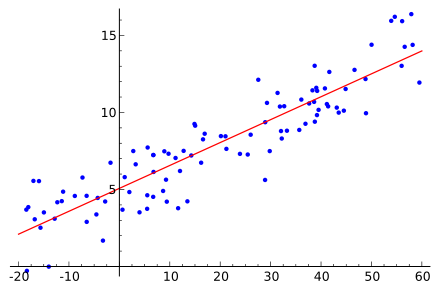
\includegraphics{./Figures/regression.png}
		\rule{35em}{0.5pt}
	\caption[Regression]{Regression: In this 1D example the data (blue dots) has one feature, plotted on the $x$-axis, with corresponding output plotted on the $y$-axis. Regression is the task of fitting some model (the red line) to the data such that a prediction can be made for any new instance with feature $x$.}
	\label{fig:regression}
\end{figure}

		\subsubsection{Classification}

Classification, as the name suggests, is assigning labels to new data having learned from examples.
Unlike regression the output, ${y}$, can only take on a discrete values.
The learning algorithm takes as a training set, $(\vo{x}_i,y_i)$, where $\vo{x}_i$ is a vector of $m$ features, $\vo{x} = (x_1, x_2, ..., x_m)$ and $y_i$ is the corresponding output\citep{domingos2012few}.
A regression model can also be used in classification problems by predicting the continuous probability of an object belonging to a class.
The output can be converted to a classification by discretization of the continuous output, like picking the class of maximum probability or thresholding.
However, there are many cases where this is impractical\citep{barber2012bayesian}.

Machine learning for classification has many useful applications.
For example, a bank can distinguish loan applicants into high-risk and low-risk groups based on spending habits.
Features relevant to a loan applicant's financial capacity can provide many weak relations associated with loan risk\citep{alpaydin2004introduction}.
A model is built from the training set of past customers' income, savings, profession, age and debt history that can predict the risk class of a new customer.
The bank uses this information to aid them in deciding if a loan should be granted.
This model is more useful than just performing classification as it also allows for knowledge extraction.
Analyzing the model that explains the data can reveal more about the underlying structure in the data and how the model recognizes differences to perform classifications.
The bank can discover attributes of low-risk customers which can help them to target advertise for new and safe loans.
% The classic example used within machine learning texts\citep{lecun2007mnist} is that of optical character recognition; recognizing printed or written characters from their scanned images.
% Handwritten characters are more interesting than printed fonts as their subtle differences in width, size, loop shapes and slants make it difficult to design a formal description of a `2' that covers all `2's and excludes all non-`2's.
% Such a character recognition system is useful in forming editable documents from scanned images and automated posting of letters from a snapshot of the address.

% Facial recognition tasks are used extensively on common platforms like the social networking website Facebook\citep{taigman2014deepface} to auto-tag friends in uploaded photos.
% This problem is significantly more difficult than optical character recognition as there are far more classes, more possible variations, larger input images and the solution must account for different orientations, lighting conditions and  facial obstructions from glasses, beards and other objects.

% Speech recognition is another classification problem with uses in popular programs such as Siri\citep{Siri} and Google Voice\citep{schalkwyk2010your}, which act as a personal assistants that can recognize spoken commands and questions.
% What makes this so challenging is the huge space in which the same word can vary in feature space.
% There are different pronunciations, accents, pitches, tones, speeds of talking and the spoken sentence must be recognized from microphone that picks up many sources of sound.




    %fraud detection\citep{domingos2012few}
%Spam filters for email are often developed through machine learning techniques, were a classifier learns to classify as spam or not.
	%[pattern recognition]

\begin{figure}[htbp]
	\centering
		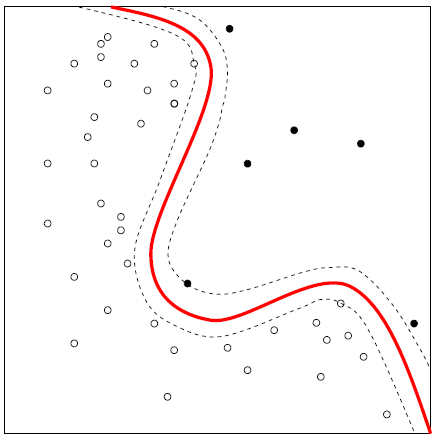
\includegraphics{./Figures/classification.png}
		\rule{35em}{0.5pt}
	\caption[Classification]{Classification: Plotted are two different classes (circles and dots) in their two dimensional feature space. Classification is the building of a model that can separate the classes such that for any new feature vector, $\vo{x}$, the class can be predicted.}
	\label{fig:classification}
\end{figure}

	\subsection{Unsupervised Learning}
    
When machine learning uses data which does not come with labels this is known as \textit{Unsupervised Learning}.
Unsupervised algorithms attempt to find structure within data without the use of labels or, put in another way, learn an accurate but compact description of the data\citep{barber2012bayesian}. 
A compact model serves as an explanation of the data that is simpler than the data itself.
The model can be used to then compress the data, requiring far less memory.

Ideally we would like machines to learn from sensor data like babies learn different objects without being explicitly told what they are.
We have yet to achieve this level of performance.
Nevertheless unsupervised learning has many applications.
A very common use is in what is known as \textit{recommender systems}\citep{domingos2012few}.
These systems are used to recommend items or advertisements that seem appropriate to the user.
You can see these systems in place on the distributer website Amazon \citep{amazon}.
After having bought or browsed items for sale, a recommender system will suggest other items for sale that users with a similar buying history to you bought themselves.
Features that will be useful here can be the items browsed, the duration of time on each, your purchase history and even your internet browsing habits picked up by cookies.

Unsupervised learning is useful for more than recommender systems.
It can be used to identify clusters in data so a company can identify the common users of its services and change its marketing strategy appropriately.
There are two main approaches to identifying clusters, generative and discriminative\citep{sammut2011encyclopedia}.
Generative assumes a parametric form of the data; that a model exists whose parameters are learned such that it could generate the data.
Discriminative borrows ideas graph theory, and works by computing a similarity matrix from the data input.
Google News searches too use this kind of machine learning \citep{das2007google}.
When a user searches for `Taiwan GDP', the engine must learn what associated links are relevant, other related links, most recent hits and popular sources without being told what to do for every possible search.


Semi-supervised learning is the common scenario in which little labeled data, but plenty of unlabeled data is available.
For example, there are many millions of images of trees on the internet, but few of those images will specify what species of tree it is.
Classifiers can still be trained on a limited amount of labeled data, if there is enough.
Semi-supervised learning takes a more advanced approach and uses the unlabeled data to enhance the classifier. 
This is generally done by narrowing in on a range of useful parameter initializations before supervised learning begins.
The motivation behind this come from the fact that when a person learns a new face, they do not have to learn what a face is altogether but just the aspects that signify the face's identity.
Unsupervised learning trains the model to be used to `seeing' trees, regardless of type, so it becomes used to their attributes even if it cannot distinguish species yet.
It will come to expect trunks, branches, green leaves and bark.
From there, the subtleties of what distinguishes one species of tree from another can then be taught using the limited labelled data.
The final model will generally be better than one trained on the labelled data alone.

\begin{figure}[htbp]
	\centering
		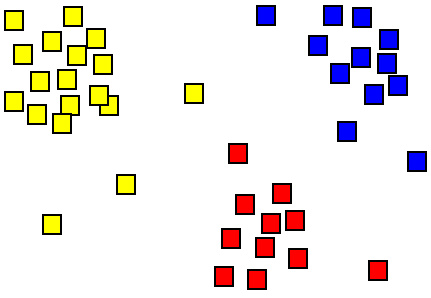
\includegraphics{./Figures/clustering.png}
		\rule{35em}{0.5pt}
	\caption[Clustering]{Clustering: Shown in a two dimensional feature space are all data instances. One application of unsupervised learning is the uncovering of structure, in this case three separate clusters of instances (highlighted by red, blue and yellow respectively).}
	\label{fig:Clustering}
\end{figure}
	\subsection{Reinforcement Learning}

Reinforcement Learning is rather different from supervised and unsupervised learning.
Instead of being given data and learning to predict output or uncover structure, reinforcement learning is given an agent and an environment.
The object is to maximize the agents behavior - its actions in particular environment states - when a reward is received over time or only at the end.
Unlike supervised learning the agent is not told ahead of time what the correct and incorrect behaviors are, and unlike unsupervised learning there is some feedback that can be used.
The concept is best illustrated in terms of a real-life creature.
To survive as long as possible - the reward - it must learn the best actions appropriate to its environment.
Some actions may have a negative impact on its lifespan, such as eating poison, while others will have a positive impact, like avoiding dangerous objects.
The reward does not have to be survival and can any long term reward.
Actions that has a positive effect are reinforced, much like training a dog with treats.

	\subsection{Online Learning}
 
Online learning, rejects the assumption made in supervised and unsupervised learning that the data $D$ is provided before the learning takes place.
Here the model must make predictions about a series of instances and it will receive a reward or loss after each one\citep{sammut2011encyclopedia}.
After each prediction and feedback the model learns from what new information was gained.
The goal is to maximize the accumulated reward, or minimize the accumulated loss.
Online learning is not uniquely supervised or unsupervised as incoming data may or may not have labels.
Expressed in a more formal manner.
For each sequence $s = 1, 2, 3, ...$, the algorithm
1) Takes input $x_s \in X$
2) Makes prediction $y_s \in Y$
3) Receives a response $z_s \in Z$
4) Incurs a loss $l_s = l(y_s,z_t)$

Online learning is similar to reinforcement learning in that appropriate predictions, rather than actions, are rewarded but the reward is instantaneous.
One common incentive for online learning is that training supervised models is often time expensive.
If you gain more data for facial recognition, a supervised model has to be trained all over again as it has no memory of what trained it before and how much it should adjust based on the new information.
Online learning however allows for the model to improve as more data comes in.
If what the model learned over time is the same as one that would be made using supervised learning using all the current data accrued, this is known as \textit{incremental learning}.

	\subsection{Anomaly Detection}
        
In anomaly detection - or outlier detection - the goal is to learn a representation of what normal data looks like.
The model generated can then be used to identify anomalies, and offer a score of the degree of abnormality\citep{barber2012bayesian}.
As regular input data does not need to be labeled, anomaly detection is an example of unsupervised learning.

The machine learning method has many useful applications.
For instance, anomaly detection is useful in the manufacturing of engines.
Having mass-produced many engines and having subjected them all to a series of quality control checks one can use anomaly detection to isolate those engines which require attention.
Another important example is that of fraudulent spending behavior or bot activity in social networks such as Twitter \citep{wang2010detecting}.

\section{Cost Functions}

The cost - also known as loss - for a prediction $y^\prime$ is a measure of relative utility of the prediction, or how different the prediction is to the correct value $y$.
The internal evaluation function , the loss function, used by the algorithm may differ from the external one we wish the classifier to optimize.

A common loss function used with classification learning is zero-one loss. 
Zero-one loss assigns  to loss for a correct classification and for an incorrect classification. 
Cost sensitive classification assigns different costs to different forms of misclassification. 
For example, misdiagnosing a patient as having appendicitis when he or she does not might be of lower cost than misdiagnosing the patient as not having it when he or she does. 

A common loss function used with regression is error squared is the square of the difference between the predicted and true values.


	\subsection{Mean Squared Error}

Mean Squared Error (mse) is a common loss function used in regression models .
It is the mean of the squared prediction errors over all examples in the test set.
The prediction error is just the difference between the true value of example $i$, $y_i$, and the predicted value, $y_i^\prime$.
\be
mse = \frac{\sum^n_{i=1}(y_i − y_i^\prime)^2}{n} 
\ee
where $n$ is the number of examples in the test set.
As the loss is proportional to the square of the difference between the prediction and true value, mse will tend to over-emphasize incorrect predictions.
This quality means the overall loss function is quite sensitive to outliers.

Similar to mse is the Mean Absolute Error (mae) given by
\be
mae = \frac{\sum_{i=1}^n abs(y_i - y_i^\prime)}{n}
\ee

	\subsection{Cross Entropy}

Cross entropy cost is appropriate to classification where the goal is to minimize the number of mis-classified training samples by imposing an exponentially increasing error the closer an output comes to being "1" when it should be "0", and vice versa\citep{mannor2005cross}.
\be
BCE = \sum^n_{i=1}[y_i ln(y_i^\prime) - (1-y_i)ln(1-y_i^\prime]
\ee

\section{Over/Under Fitting, Variance and Bias}

The main goal with machine learning is to generalize beyond the example data given in the training set.
It would be easy to guarantee 100\% percent success with a machine learning algorithm on just the training data.
The data could just be memorized by the algorithm and when any of the example input vectors are fed to the classifier it will score perfectly.
As an analogy; if you only studied for a test by doing learning how to answer questions in past papers you are sure to do incredibly well should those questions appear.
However you have sacrificed general knowledge of the subject for knowing those particular questions.
Should the exam have questions you have not seen before you will likely perform poorly \citep{flach2012machine}.
In machine learning terms you were \textit{over-fitting} to the training set, the past papers, and were not generalizing well to perform well on the test set.

This illustrates the need for splitting all the data you have into a training and test set.
It is important that the training and test samples are representative of the underlying problem.
The test set must not in any way be used to create a classifier.
Should it be used for training then your model can learn to fit the test set; like a student learning to pass a particular test and not be generally good at the subject.
This idea of over-fitting suggests the surprising result that it is often better not to fully optimize the model fit to the training data.
Over-fitting can occur quite easily in regression problems where the output is dependent on more than the information contained in the data set, like environmental noise.
Should your model fit the training set too well it is essentially fitting to the noise and not to the general trend.

As a rule of thumb it is best to have far less model parameters than training examples.
The issue of over and under-fitting can also be described in terms of bias and variance.
To illustrate, if you have three spread data points on an $X-Y$ axis to which you fit a straight line it will likely not be a good fit.
The model has insufficient complexity - loosely the number of parameters - to model the data, it has a high bias.
The model fitted is far too general, much like fitting a horizontal line to equidistant data points generated from a sine graph.
True, a sine function oscillates around $y=0$ but a straight line fit will not capture the oscillatory behavior at all. 
If we underestimate the number of parameters of the model, we will not be able to fit well, regardless of how much training data we have, we have \textit{under-fit}.
As there are more than two points, a 2nd degree polynomial, a parabola, will likely fit better.
A multinomial can be made directly through all three points, but may introduce wiggles that seem unnatural.
Taking the example to the extreme, a hundred degree polynomial has an infinite number of ways of modeling the three points but most of those will have a large variance, that is unnecessary `wiggle'.
A model with too many degrees of freedom will be too sensitive to the training sample, and small variations in the training sample can result in a considerably different model. 
This trade-off phenomenon is know as the \textit{bias–variance dilemma}: a low-complexity model suffers less from variability from random variations in the training data, but may introduce a systematic bias that even large amounts of data cannot resolve; on the other hand, a high-complexity model eliminates such bias but can suffer non-systematic errors due to variance in the data.

\begin{figure}[htbp]
	\centering
		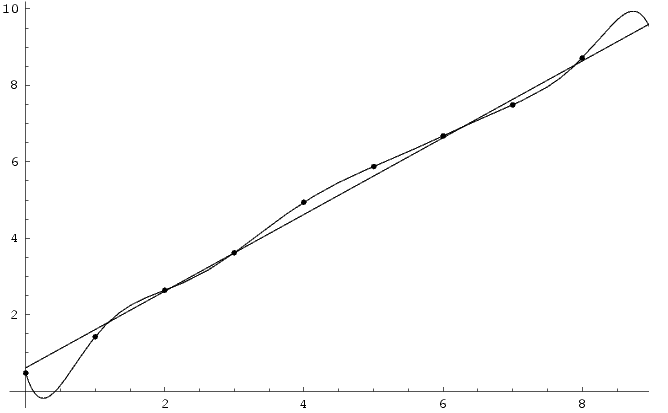
\includegraphics{./Figures/overfit.png}
		\rule{35em}{0.5pt}
	\caption[Over-fitting]{Over-fitting: Data, represented by points, is plotted with the $x$-axis representing the single feature and the $y$-axis to the corresponding output. A model that fits well will capture the general surface, like the straight line in this example. An 8th order polynomial (the curved line) can be made to go through all the data exactly but introduces unreasonable predictions like the bumps on the top right and bottom left. It is said to be over-fitting the data. }
	\label{fig:over-fitting}
\end{figure}

Another important aspect of generalization is this.
Data alone may never be enough, regardless of how much you have\citep{domingos2012few}.
Consider the case of a boolean function with 100 parameters from a million examples.
There are $10^6$ examples whose class you do not know.
In the absence of further information there is no method of classification that would beat flipping a coin.
Every algorithm must make use of some knowledge about the data, or make some assumptions beyond what is given in order to generalize.
This `no free lunch' theorem was formalized by Wolpert which stipulates that no algorithm, can beat random guessing over all possible functions to be learned\citep{Wolpert96thelack}.
This seems to drown out any possibility for machine learning to be effective in the real world.
On closer inspection however, the functions we want to learn in the real world are not drawn uniformly from the set of all mathematically possible functions.
We make assumptions such as smoothness, similar examples having similar classes, limited dependencies and favour mathematical functions that are less complex.
This has to do with the difference between deduction and induction.
Through deduction, deriving results from assumed axioms, we are very limited in what we can deduce from data.
In comparison, induction, what Sherlock Holmes actually does, we can turn a small amount of input data into models that generalize very well if not necessarily all the time.
	\subsection{Regularization}
    
If the model has more parameters than necessary it will tend to over-fit the training data\citep{goyal2014object}.
\textit{Regularization} is the process of ensuring over-fitting does not occur.
The simplest method is to add a penalty term to the error.

\be
E(W) = \frac{1}{n}\sum^n_{i=1} e_i =\frac{1}{n}\sum^n_{i=1}(y_i - y_i^\prime)^2
\ee
\be
\widetilde{E}=E(W) + \frac{\lambda}{2}W^T W
\ee
where $E$ is the Mean Square Error as a function of the parameters weightings (values) $W$, $y_i$ are the correct labels, $y_i^\prime$ the predicted labels, $\lambda$ is a constant given before learning and $\widetilde{E}$ is the modified error with the addition of a penalty term.
Mean Squared Error is the base loss used in this example but regularization terms can be added to any loss function.
Now as the weights increase in value of the regularization term will increase.
The model is thereby punished for utilizing parameters by the added cost, the more parameters used and the larger the weights the greater the cost will be from the regularization term\citep{goyal2014object}.
In order to minimize the loss, the model is now encouraged to fit the training data as before and to do so with the fewest parameters.

Lambda is an example of a hyper parameter, which is a variable that guides the learning algorithm in its operation.
Common to many learning algorithms is the learning rate which affects how fast the model learns.
It is important to find the appropriate hyper-parameters for the problem at hand as they can effect the speed at which learning happens and the ultimate success of the model built.
So how do you decide the value of $\lambda$, or how much to value the regularization cost?
That we will cover in the next section.


        \subsection{Validation}

It is not enough to split the data into training and test sets to avoid avoid over-fitting.
The practitioner cannot tune hyper parameters by seeing which values lead to the best performance on the set set.
To do this is effectively training on the test data and it is no longer an independent source of data with which to evaluate your model\citep{witten2005data}.

This concern is what motivates the split of all the data into a training, cross-validation and test set.
Commonly a validation set, $D_{valid}$ is made by splitting the complete data $D$ into two parts, $D_{train}$ and $D_{valid}$.
The validation set is routinely chosen to be smaller than the training set so that the majority of the data is used in training.
There is no absolutely correct ratio for the validation/training split, however it is common practice to split the data 70/30 for training and validation sets respectively.

If regularization is used there will be a regularization parameter $\lambda$ that can take on many values.
The best lambda value (or any other hyper parameter) can be found by exploring the range of possible values and comparing the resultant models.
The hyper parameters that result in the best performance on the validation set, $D_{valid}$, are chosen.
Then the model is finally tested on the test set for its unbiased performance evaluation.

To summarize: training is done on the training set, fine-tuning of parameters on the cross-validation set and the final performance measure will be on the test set\citep{barber2012bayesian}.

Once the hyper parameters have been selected and the model is tested on the set set, it is alright to then include the test and validation sets along with the training set to then retrain the model with all the data.
With some well-behaved learning methods this is a reliable method to enhance the model\citep{witten2005data}.
However to evaluate this new model a new source of test data must be created altogether.


	\subsection{Cross Validation}

Of course, all this splitting of the data reduces that available for training.
A further difficulty is that the less data used for testing the less reliable are the error estimates on the models accuracy.
There are multiple approaches to how this trade-off problem is handled.
One method is to partition the data randomly into training and validation sets multiple times.

\begin{figure}[htbp]
	\centering
		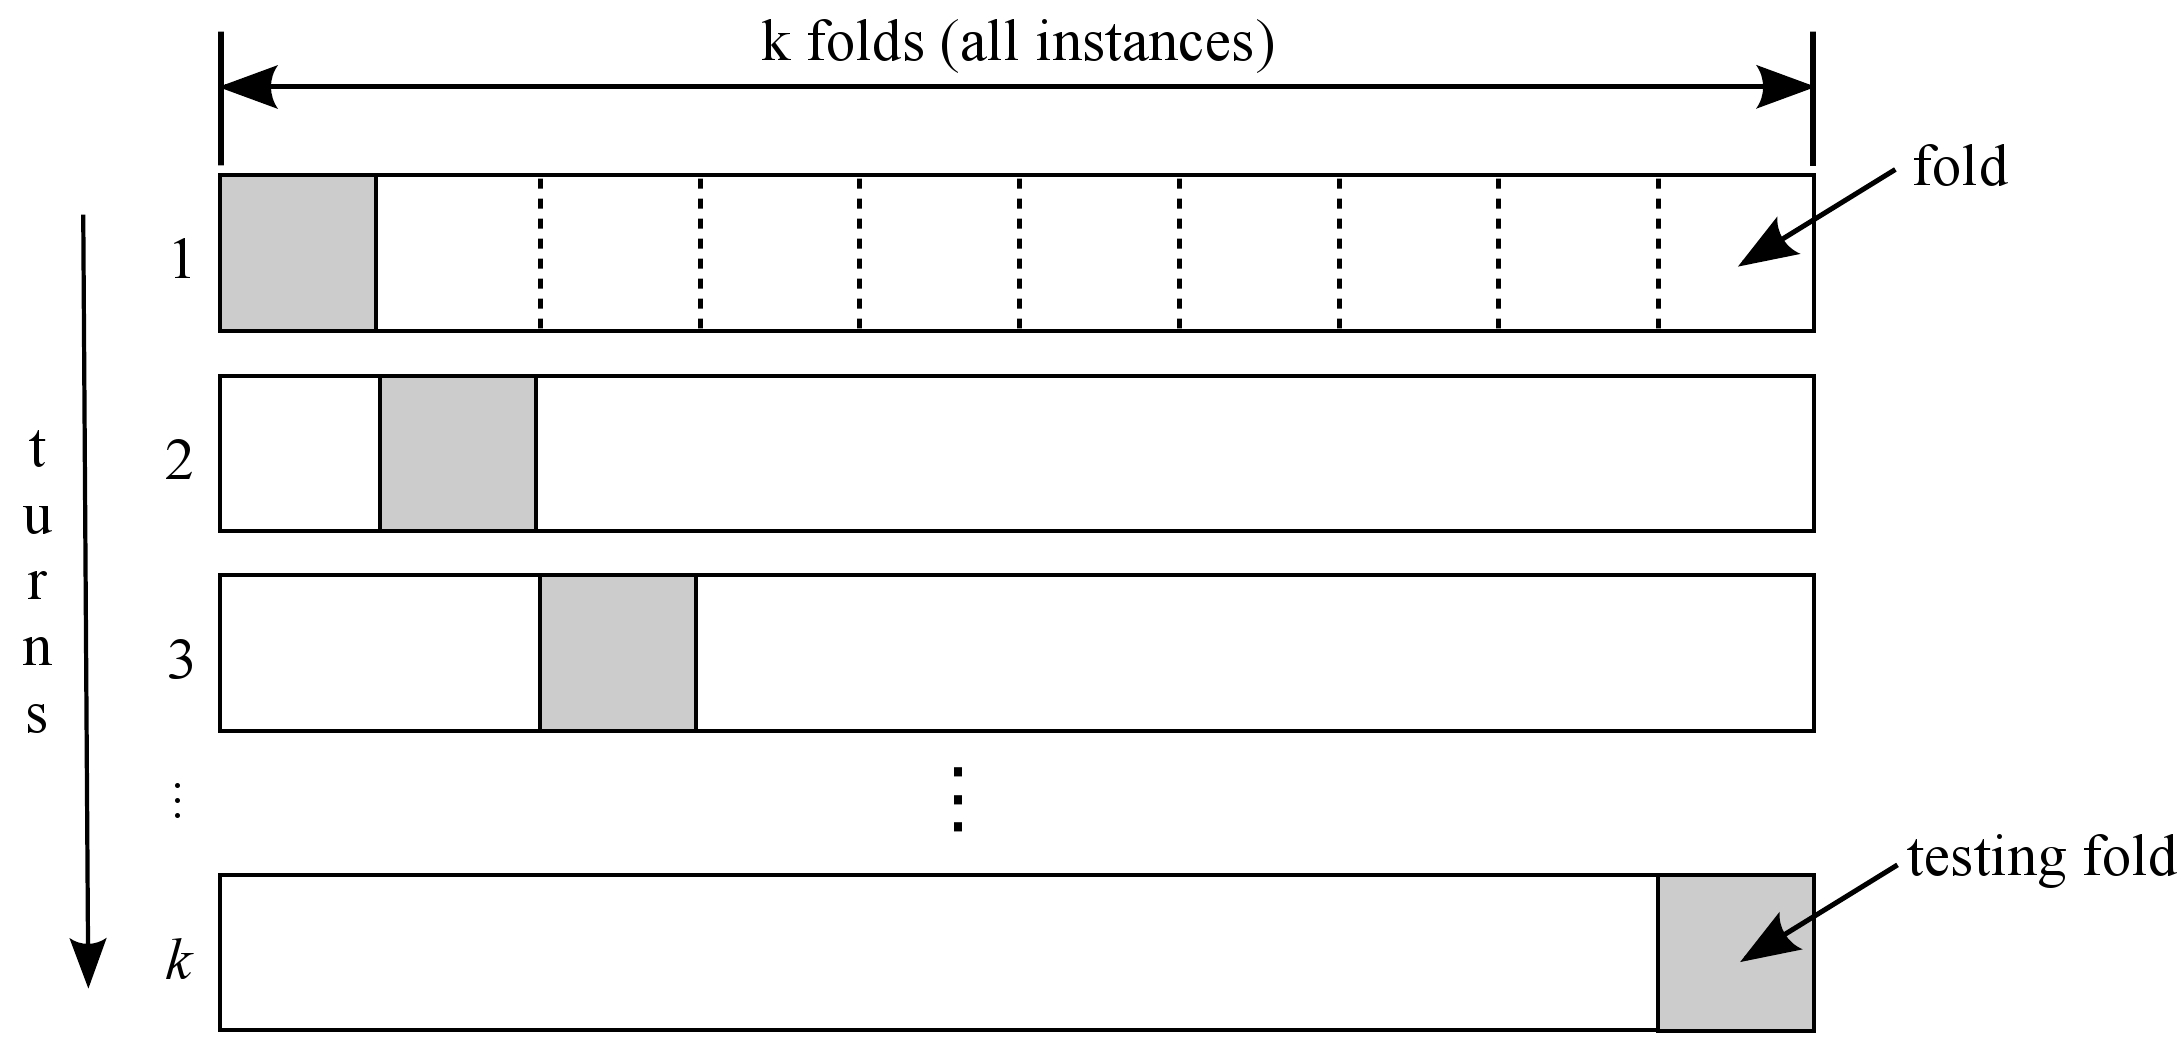
\includegraphics{./Figures/k_fold_validation.jpeg}
		\rule{35em}{0.5pt}
	\caption[k-fold Validation]{K-fold validation: The total data set is split into $k$ pieces. The model is then trained using all but 1 piece of the data which is the validation set. This is done $k$ times where the withheld validation set is a different for every run.}
	\label{fig:k_fold_validation}
\end{figure}

A common method of doing this is $K$-fold cross validation which is particularly useful when there is not much data to begin with\citep{barber2012bayesian}.
The total data is split into $K$ equal sized  partitions so there are now $K$ potential validation sets.

The model is trained on the $K-1$ partitions, leaving out the $K$'th piece as the validation set.
This will be repeated for all possible training set combinations and the validation success will be measured by the average of all $K$ validation performances.
The average of all these results is used for fixing the hyper parameters,
In practice many machine learning practitioners use 10-fold validation.
As before the model's true prediction error should be tested on an entirely unused test data set.

\section{Performance Measures}

It may be quite intuitive to think a model's success can be measured by accuracy alone however this does not tell the whole story.
 
	\subsection{Test performance Error}

If we measure a model to have an accuracy of $85\%$ this does not tell us how much the true value may differ with different degrees of confidence.
We would be more confident of the accuracy being near the $85\%$ if we got that result from a test set of 10,000 instances than of 100.
We consider the test to be like a Bernoulli process in order to give some measure of confidence
In statistics, a Bernoulli process is one in which a succession of independent events can have one of two results, like pass and fail, correct or not. 

This has a simple method for providing confidence intervals\citep{witten2005data}.
\be
p \pm z \sqrt{\frac{1}{n} p(1-p)}
\ee
where $p$ is the accuracy estimated from the test set, $z$ is the $1-\frac{1}{2}\alpha$ quantile often given in the back of many statistical textbooks, and $n$ is the number of samples within the test set.
For the commonly used confidence level of $95\%$ the value for $z$ is $1.96$.

	\subsection{Confusion Matrix} 
    
If we have a classification model and give it a test instance, there are four possible outcomes. 
If the instance is positive and the model predicts positive, it is called a true positive (TP); if classified as negative, it is a false negative (FN). 
On the other hand if an instance is negative and classified as negative, it is a true negative (TN); but if classified as positive, it is a false positive (FP). 

We can construct a confusion matrix, also called a contingency table, with the outcomes from the test set.
Each row in the table refers to the true classes as recorded in the test set, and each column to classes as predicted by the classifier\citep{flach2012machine}. 

\begin{figure}[htbp]
	\centering
		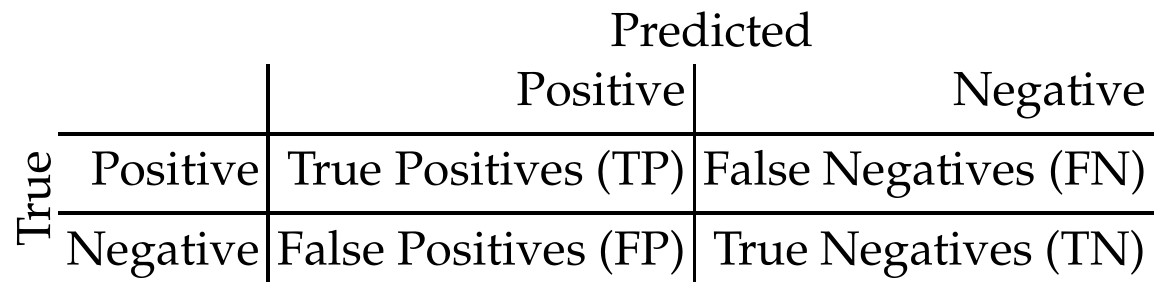
\includegraphics{./Figures/confusion_matrix.jpg}
		\rule{35em}{0.5pt}
	\caption[Confusion Matrix]{A confusion matrix encapsulates the success of a classification model. Rows refer to the true classes, columns to the models predictions of those examples.
	If correctly classified as Positive/Negative it is a True Positive/Negative. Otherwise it is False Positive/Negative.}
	\label{fig:confusion_matrix}
\end{figure}

From the confusion matrix we can calculate a range of performance metrics. 
Accuracy is the simplest which you are already familiar with
\be
Accuracy = \frac{TP+TN}{TP +TN+FP+FN}
\ee

	\subsection{Precision and Recall}
        
        
        
Two useful measures of classification performance are completeness and efficiency\citep{flach2012machine}
These two measures are defined from the outcomes on the confusion matrix\citep{ball2010data}.

Completeness (also known as Recall, Sensitivity or True Positive Rate (tpr)) is the fraction of objects truly belonging to a category that are classified correctly,

\be
Completeness = Recall = Sensitivity = tpr = \frac{TP}{TP+FN} 
\ee

The False Positive Rate(fpr) or `Type 1 error' is given by
\be
fpr = \frac{FP}{FP + TN}
\ee
which relates to the Specificity,
\be
Specificity = \frac{TN}{FP + TN} = 1 -fpr 
\ee
Precision (also known as Efficiency) is the fraction of objects classified as a class that truly belong to that class:
\be
Efficiency = Precision = \frac{TP}{TP+FP} 
\ee

The ideal would be to have both precision and recall to be close to one, however there is often a trade-off between the two.
The preferred balance will be problem dependent and may hinge on not having too much contamination of positive, or the economic costs of incorrect classifications etc.
For example, if you wish to find as many positive examples as possible, requiring high recall, this will come at the cost of contamination, or lower Precision.
However, if you wish to more confident of the objects classified and are willing miss some instances than a high Precision is important at the expense of Recall.

In practice Precision and Recall are particularly important measures in the case of skewed classes.
Skewed Classes is a problem in which one class is significantly outnumber the other class or classes in the data set.
If you are detecting fraudulent behavior in online banking, the majority of activity will be normal.
Should a classier predict the activity is normal all the time (clearly a bad classifier) it will still be right most of the time and score a high accuracy.

	\subsection{F-measure}
    
A measure that combines precision and recall to give an indication of the algorithm's success is the $F_\beta$ measure (for real non-negative values of $\beta$)\citep{sokolova2006beyond}\citep{davis2006relationship}:
\be
F_\beta=\left(1+\beta^2\right)\frac{precision.recall}{\beta^2.precision + recall}
\ee
The F-score favours Precision when $\beta > 1$, is evenly balanced when $\beta = 1$ and favours Recall where $\beta < 1$.
When balanced we have the F-measure or balanced F-score
\be
F_1=2\frac{precision.recall}{precision +recall}
\ee
with a range of zero to one.

	\subsection{ROC Curve and AUC Score}
     


The Receiver Operating Characteristic (ROC) graph is an encompassing visualization of a binary classifiers performance \citep{fawcett2006introduction} \citep{davis2006relationship} \citep{sokolova2006beyond}.
They have long been used in signal detection theory as a way of visualizing and evaluating the trade off between false alarms and correct hits.
It has been used commonly in medicine in the design of diagnostic tests which are not 100\% accurate.
As mentioned when discussing Precision and Recall, accuracy does not paint a full picture of the models performance.
To understand thus picture a database of skew classes - classes in which one category is far more abundant than another - with 90\% cat images and 10\% dogs.
The model can score 90\% accuracy simply by guessing `cat' every time.
If you accepted this accuracy at face value you might conclude the model is fantastic at distinguishing between the two classes when in fact it could never recognize a dog.
ROC curves are useful even in cases even where there are no class imbalances because they allow for better analyzing the trade-off between the false positive rate and the true positive rate.
        
Consider a case of two classes.
Formally each example $E$ is mapped to one of the set $\{p,n\}$ which are positive and negative labels respectively.
The classier or model is a mapping from each example to one of the classes.
Some models will do this by producing continuous output, say a number between $0$ and $1$, to which threshold is applied.
If the output surpasses the threshold it is classified as $1$, for positive, otherwise $0$ for negative.
Some models themselves output a discrete class label, for this example $0$ or $1$.

The ROC curve is a plot of tpr on the Y-axis vs fpr on the X-axis.
For a model that produces continuous output, by changing the threshold you can obtain many pairs of (tpr,fpr) values which will produce a curve on the ROC graph.
For a model that has discrete output, even before any threshold, this will only be a single point on the graph corresponding to the only (tpr,fpr) pair.
Such discrete scoring classifiers can often have their internal state converted into a score rather than a discrete outcome which will provide a full ROC curve.
An example of this is in the decision tree algorithm that produces its discrete output based on the proportion of one instance over another at the final node.
By just using the ratio, and not choosing the most common label you have a continuous score.

The ideal model should go through the point (0,1), that is where there are no false positives and a 100\% true positive rate.
Classifiers that appear toward the the left hand side of the plot can be thought of as conservative, in that they require strong evidence to make a positive classification. 
Because they are so stringent few examples will be classified as positive.

Classifiers appearing toward the upper right are quick to label an example as positive, so they are likely not to miss positive classifications.
Their lax criteria will however likely contaminate the pool of positives with many incorrectly labelled negatives.

As there are generally more negative cases than positive, more non-cats then cats, behavior of the ROC curve toward the upper left tends to be the most informative.

If a models ROC curve lies along the 45 degree $y=x$ line it means the classifier is either randomly guessing, or that the model has not learned any useful representation of the data and has no better prediction than random guessing.
If it guesses positive half of the time it will have a tpr equal to 0.5, however now half of the negatives will be incorrectly classified the fpr will equal 0.5 as well.
This $y=x$ trend will be true for any percentage of a random example being positive, yielding a line along $y=x$.
In fact, if the proportion of positive to negative classes changes an ROC curve will not be affected at all.
This is part of What makes ROC curves so useful.
Classes that outnumber their opposite class are very common in real world problems making a performance measure invariant to skewness even more valuable.
In some cases the skewness of classes may alter with time, such as the number of diseased people, but that does should not change the fundamental characteristics of what identifies someones as part of the class

Should a model appear below the $y=x$ line this means it performs even worse than random guessing.
However, should label predictions be swapped around the point will end up in the top left.
This means the model does capture some information about the classes, but is using it incorrectly.


It will often be the case that the most natural threshold of $0.5$ for a model output between $0$ and $1$ is not the best.
Depending on the model and the problem it may be that selecting the threshold to be 0.6 has a better trp without increasing the fpr.

As continuous models may produce output between different values, 0 to 1 and -1 to 1, it is not possible to compare the the models at equivalent threshold to see their performance.
In fact, even when their output range is the same, they are still not comparable at equivalent thresholds as the output scores are relative, not proper probabilities.
Another way of saying this, is that the scores are not properly calibrated.

\begin{figure}[htbp]
	\centering
		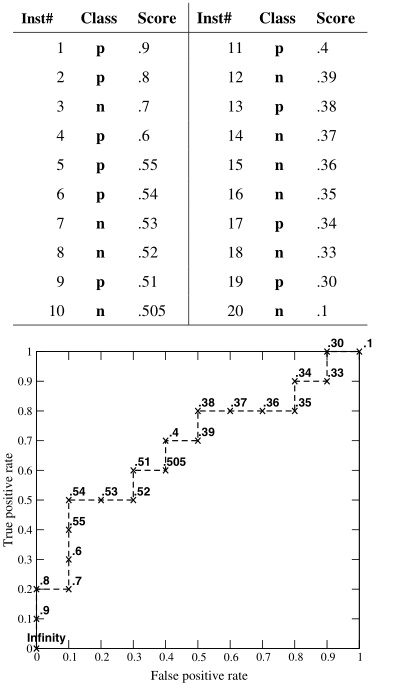
\includegraphics{./Figures/ROC_curve.png}
		\rule{35em}{0.5pt}
	\caption[ROC Curve]{ROC Curve: The model scores vary between 0 and 1. The threshold(shown above the crosses) is varied over all score values in the test set and the true positive rate (tpr) and false positive rate (fpr) you can produce the 2D ROC curve.}
	\label{fig:roc_curve}
\end{figure}



A common way of comparing models to each other in a single measure is to use the Area Under an ROC Curve (AUC).
A perfect classifier would reach a tpr of 1 and fpr of 0, so the curve would be a straight line along $tpr=1$ with an area underneath of 1.
A classifier that performs no better than random would score half of the total area, $0.5$.
It is still possible for a model of low AUC curve to perform better than its high AUC curve in a particular region, but the AUC implies it is inferior over all.
Therefore one should not necessarily select the model with the highest AUC score as it depends on the costs of making a true positive and a false negative.
For example, if astronomers make a classifier of abnormal galaxies in order to follow them up with further study, it is more important to have a high true positive rate, even at the risk of weeding out some, than it is to have a low true positive rate but high false positives.
IF there are a large number of false positives the data set is essentially contaminated with a large pool of galaxies the astronomers cannot afford telescope time to waste on. 
Here fewer positives of high quality is better than many positives of low quality.
So if a model happens to perform best in the ROC region of interest even though it has lower AUC score it would be the `economical' choice.
In addition to this `economics' problem, selecting the model with the highest AUC score from a single test score is very similar to selecting the model with the highest test accuracy.
Without a measure of the variance this score can only be trusted so much.
This can be done by testing on multiple test sets, generated via cross-validation or bootstrapping (covered in Model Ensembles) and then averaging.
There exist multiple methods for averaging ROC curves that preserve information of interest.
Multiple class/dimension ROC curves can be made for where there are more than two classes, although this is uncommon and can be difficult to analyze.
Methods exist to obtain a desired tpr/fpr performance that lies between two models ROC curves.
These methods are can all be found in the main source for this section \citep{fawcett2006introduction} on ROC curves, but are beyond the needed scope of this masters  .

\section{Model Ensembles}

Empirical observations show that the best machine learning algorithm to use depends on the application\citep{domingos2012few}.
Combining many different models often produces much better results than a single algorithm could achieve alone \citep{witten2005data}.
There are pathological cases in which an ensemble of models can actually perform worse than any of the models individually, however that will seldom be the case in real world problems.
Model ensembles can be made with many methods, the two most common being; Bagging and Boosting.

Bagging is one of the simplest techniques.
Each member of the ensemble is constructed from a different training dataset.
A different dataset is generated by sampling from the total $N$ data examples, randomly choosing $N$ items with replacement.
Each set is known as a bootstrap.
The name Bagging is derived from an acronym of Bootstrap AGGregatING \citep{hothorn2003double}. 
As items are selected with uniform likelihood and replacement the probability of a single data item not being selected is $p = (1−\frac{1}{N})^N$ 
For large $N$, a single bootstrap will likely contain 63.2\% of the complete set.
The net result of Bagging is greatly reducing the variance while increasing bias by only a little.

From here it is as simple as having the multiple classifiers cast votes on the final output.
That said, instead of taking votes from the discrete outcomes, it often makes more sense to average the continuous output used to create the individual labels.
These are often more accurate and can often be used to produce probability estimates as well.
For a regression problem the average output of the models is used.
Models are given equal weight for both voting and averaging in Bagging\citep{witten2005data}.

Bagging can be done with just one learning algorithm, provided the algorithm is unstable.
An unstable algorithm is one that produces a different model each time with just a small change to the training data.
The reason for this is that several machine learning algorithms have some element of randomness, such as randomly initialized weights or randomness introduced in training, which likely results in different classifiers.
These are also known as high variance models, common examples being decision trees and neural networks.
As such Bagging does not work well with linear models because bootstrap sampling will produce almost identical (low diversity) models.
Many non-random models can have an element of randomness introduced, which often has the drawback of making the individual model worse, but the ensemble generally benefits.
One difficulty with Bagging is that the resultant model ensembles are particularly hard to analyse to understand their internal workings.


Boosting is really a family of model ensemble techniques.
Here training samples have weights and these are altered so that each new classifier focuses on examples the previous classifier tends to get wrong\citep{witten2005data}.
In this way the method seeks multiple models that complement each other.
Unlike bagging this process is iterative, each new model is influenced by the performance of previous models\citep{witten2005data}.
Finally Boosting also gives models a different weighting when voting or averaging to reflect the confidence of each model.
Adaboost is the most well known and successful of the Boosting techniques though there are many others.
Some Boosting techniques are designed to be specialized for being cost-sensitive and noise-tolerant.
